\documentclass{exercise}

\institute{Applied and Computational Mathematics}
\title{Selbstrechenübung 5}
\author{Joshua Feld, 406718}
\course{Mathematische Grundlagen IV}
\professor{Torrilhon \& Berkels}
\semester{Sommersemester 2022}
\program{CES (Bachelor)}

\begin{document}
    \maketitle


    \section*{Aufgabe 1}
    
    \begin{problem}
        Gegeben sei das glatt berandete Gebiet \(\Omega\) wie in der folgenden Abbildung mit den Rändern \(\Gamma_1\) und \(\Gamma_2\).
        Gesucht wird eine Funktion \(u \in C^2\parentheses*{\Omega}\) mit
        \begin{align*}
            -\Delta u\parentheses*{x} &= 0, \quad x \in \Omega,\\
            u\parentheses*{x} &= 1, \quad x \in \Gamma_1,\\
            u\parentheses*{x} &= 0, \quad x \in \Gamma_2.
        \end{align*}
        \begin{center}
            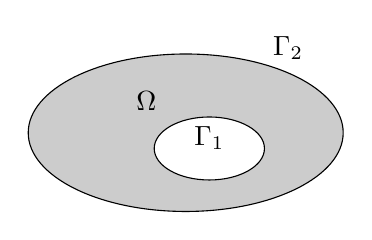
\begin{tikzpicture}
                \draw[fill=white!80!black] (0,0) ellipse (2cm and 1cm);
                \draw[fill=white] (.3,-.2) ellipse (.7cm and .4cm);
                \node[anchor=north] at (.3,.2) {\(\Gamma_1\)};
                \node[anchor=south] at (1.3,.8) {\(\Gamma_2\)};
                \node at (-.5,.4) {\(\Omega\)};
            \end{tikzpicture}
        \end{center}
        \begin{enumerate}
            \item Zeigen Sie, dass \(u\) auf \(\Omega\) beschränkt ist, und geben Sie eine untere und eine obere Schranke an.
            \item Zeigen Sie
            \begin{align*}
                \partial_n u &= \nabla u \cdot n \ge 0\text{ auf }\Gamma_1,\\
                \partial_n u &= \nabla u \cdot n \le 0\text{ auf }\Gamma_2,
            \end{align*}
            wobei \(n\) der äußere Normalvektor auf \(\Gamma_1\) bzw. \(\Gamma_2\) ist.

            \emph{Hinweis: \(\partial_n u = \lim_{h \to 0}\frac{1}{h}\parentheses*{u\parentheses*{x} - u\parentheses*{x - hn}}\)}
        \end{enumerate}
    \end{problem}
    
    \subsection*{Lösung}
    \begin{enumerate}
        \item Da \(u \in C^2\parentheses*{\Omega}\) und \(u\) harmonisch ist, nimmt \(u\) sein Maximum am Rand an (Maximumprinzip), d.h.
        \[
            u\parentheses*{x} \le 1, \quad x \in \Omega.
        \]
        Für \(w\parentheses*{x} = -u\parentheses*{x}\) gilt
        \begin{align*}
            \Delta w &= 0 \quad \text{in }\Omega,\\
            w &= -1 \quad \text{auf }\Gamma_1,\\
            w &= 0 \quad \text{auf }\Gamma_2.
        \end{align*}
        Da auch \(w \in C^2\parentheses*{\Omega}\) und harmonisch ist, nimmt \(w\) sein Maximum am Rand an, d.h.
        \[
            w\parentheses*{x} \le 0 \quad x \in \Omega,
        \]
        also
        \[
            u\parentheses*{x} \ge 0 \quad x \in \Omega.
        \]
        \item Für die Normalableitung gilt
        \[
            \partial_n u\parentheses*{x} = \nabla u\parentheses*{x} \cdot n = \lim_{h \to 0}\frac{1}{h}\parentheses*{u\parentheses*{x} - u\parentheses*{x - hn}}.
        \]
        Für \(x \in \Gamma_2\) ist \(u\parentheses*{x} = 0\), und da \(x - hn\) in \(\Omega\) liegt (für kleine \(h\)), ist \(u\parentheses*{x - hn} \ge 0\) und folglich
        \[
            \partial_n u\parentheses*{x} = \lim_{h \to 0}\frac{1}{h}\parentheses*{u\parentheses*{x} - u\parentheses*{x - hn}} \le 0.
        \]
        Für \(x \in \Gamma_1\) ist \(u\parentheses*{x} = 1\).
        Da auch hier \(x - hn\) in \(\Omega\) liegt (für kleine \(h\)), ist \(u\parentheses*{x - hn} \le 1\) und folglich
        \[
            \partial_n u\parentheses*{x} \ge 0.
        \]
    \end{enumerate}


    \section*{Aufgabe 2}
    
    \begin{problem}
        Betrachten Sie das Randwertproblem für Konstanten \(c_1, c_2 \in \R\)
        \begin{align*}
            -u''\parentheses*{x} - c_1 u\parentheses*{x} &= 0, \quad x \in \parentheses*{0, 1},\\
            u\parentheses*{0} &= 0,\\
            u\parentheses*{1} &= c_2.
        \end{align*}
        \begin{enumerate}
            \item Bestimmen Sie das Gleichungssystem
            \[
                Au_h = b,
            \]
            mit \(A \in \R^{n \times n}\) und \(b \in \R^n\), das sich aus einer Diskretisierung der Differentialgleichung mit zentralen finiten Differenzen zweiter Ordnung für \(u''\) mit der Schrittweiter \(h = \frac{1}{n + 1}\) ergibt.
            \item Zeigen Sie, dass die Matrix \(A\) die Eigenwerte
            \[
                \lambda_k = \frac{4}{h^2}\sin^2\parentheses*{\frac{k\pi h}{2}} - c_1, \quad k = 1, \ldots, n
            \]
            und die zugehörigen normierten Eigenvektoren
            \[
                v_k = \sqrt{2h}\parentheses*{\sin\parentheses*{k\pi h}, \sin\parentheses*{2k\pi h}, \ldots, \sin\parentheses*{nk\pi h}}^T
            \]
            besitzt.
            \item Lösen Sie das Gleichungssystem für \(c_1 := \pi^2\) mit dem Ansatz
            \[
                u_h = \sum_{i = 1}^n \alpha_i v_i
            \]
            und bestimmen Sie die Koeffizienten \(\alpha_i\) durch geeignete Skalarprodukte.
            Prüfen Sie, ob der so berechnete Ausdruck für \(\alpha_i\) wohldefiniert ist.

            \emph{Hinweis: Für \(x \in \left(0, 1\right]\) gilt \(\arcsin\parentheses*{x} < \frac{\pi}{2}x\).}
            \item Zeigen Sie für \(c_1 := \pi^2\) und \(c_2 > 0\), dass die erste Komponente \(u_1\) der Lösung \(u_h\) für \(h \to 0\) gegen \(-\infty\) divergiert.

            \emph{Hinweis: Verwenden Sie die Taylorentwicklungen
            \begin{align*}
                \sin^2\parentheses*{ah} &= a^2 h^2 - \frac{1}{3}a^4 h^4 + \mathcal{O}\parentheses*{h^6},\\
                \sin\parentheses*{ah}\sin\parentheses*{a\parentheses*{1 - h}} &= ah\sin\parentheses*{a} - a^2 h^2 \cos\parentheses*{a} + \mathcal{O}\parentheses*{h^3}.
            \end{align*}}
            \item Was lässt sich über die analytische Lösung des Randwertproblems für \(c_1 := \pi^2\) sagen?
        \end{enumerate}
    \end{problem}
    
    \subsection*{Lösung}
    \begin{enumerate}
        \item Finite Differenzen für die zweite Ableitung
        \[
            u''\parentheses*{x} = \frac{u\parentheses*{x + h} - 2u\parentheses*{x} + u\parentheses*{x - h}}{h^2} + \mathcal{O}\parentheses*{h^2}
        \]
        liefern das Gleichungssystem \(Au_h = b\) mit
        \[
            A = \frac{1}{h^2}\begin{pmatrix}
                2 & -1 & 0 & \cdots & 0\\
                -1 & \ddots & \ddots & \ddots & \vdots\\
                0 & \ddots & \ddots & \ddots & 0\\
                \vdots & \ddots & \ddots & \ddots & -1\\
                0 & \cdots & 0 & -1 & 2
            \end{pmatrix} - c_1 \cdot I_{n \times n} \quad \text{und} \quad b = \frac{1}{h^2}\begin{pmatrix}
                0\\\vdots\\0\\c_2
            \end{pmatrix}.
        \]
        \item Prüfe, ob \(Av_k = \lambda_k v_k\):
        \begin{align*}
            Av_k &= \parentheses*{\frac{1}{h^2}\begin{pmatrix}
                2 & -1 & 0 & \cdots & 0\\
                -1 & \ddots & \ddots & \ddots & \vdots\\
                0 & \ddots & \ddots & \ddots & 0\\
                \vdots & \ddots & \ddots & \ddots & -1\\
                0 & \cdots & 0 & -1 & 2
            \end{pmatrix} - c_1 \cdot I_{n \times n} \quad \text{und} \quad b = \frac{1}{h^2}\begin{pmatrix}
                0\\
                \vdots\\
                0\\
                c_2
            \end{pmatrix}} \cdot \begin{pmatrix}
                \sin\parentheses*{k\pi h}\\
                \sin\parentheses*{2k\pi h}\\
                \vdots\\
                \sin\parentheses*{nk\pi h}
            \end{pmatrix}\sqrt{2h}\\
            &= \begin{pmatrix}
                \parentheses*{2\sin\parentheses*{k\pi h} - \sin\parentheses*{2k\pi h}} \cdot \frac{\sqrt{2h}}{h^2} - c_1\sin\parentheses*{k\pi h} \cdot \sqrt{2h}\\
                \parentheses*{-\sin\parentheses*{k\pi h} + 2 \sin\parentheses*{2k\pi h} - \sin\parentheses*{3k\pi h}} \cdot \frac{\sqrt{2h}}{h^2} - c_1\sin\parentheses*{2k\pi h} \cdot \sqrt{2h}\\
                \vdots\\
                \parentheses*{2\sin\parentheses*{nk\pi h} - \sin\parentheses*{\parentheses*{n - 1}k\pi h}} \cdot \frac{\sqrt{2h}}{h^2} - c_1\sin\parentheses*{nk\pi h} \cdot \sqrt{2h}
            \end{pmatrix}
        \end{align*}
        Hier genügt es folgende Gleichung zu vereinfachen (\(j = 1, \ldots, n\)):
        \begin{align*}
            &\frac{\sqrt{2h}}{h^2}\parentheses*{-\sin\parentheses*{\parentheses*{j - 1}k\pi h} + 2\sin\parentheses*{jk\pi h} - \sin\parentheses*{\parentheses*{j + 1}k\pi h}} - c_1\sin\parentheses*{jk\pi h}\sqrt{2h}\\
            &= \frac{\sqrt{2h}}{h^2}\left(-\parentheses*{\sin\parentheses*{jk\pi h}\cos\parentheses*{k\pi h} - \cos\parentheses*{jk\pi h}\sin\parentheses*{k\pi h}} + 2\sin\parentheses*{jk\pi h}\right.\\
            &\left.-\parentheses*{\sin\parentheses*{jk\pi h}\cos\parentheses*{k\pi h} + \cos\parentheses*{jk\pi h}\sin\parentheses*{k\pi h}}\right) - c_1\sin\parentheses*{jk\pi h}\sqrt{2h}\\
            &= \underbrace{\sqrt{2h}\sin\parentheses*{jk\pi h}}_{:= \parentheses*{v_k}_j}\parentheses*{\frac{2 - 2\cos\parentheses*{k\pi h}}{h^2} - c_1}\\
            &= \parentheses*{v_k}_j\parentheses*{\frac{2}{h^2}\parentheses*{1 - \cos\parentheses*{k\pi h}} - c_1}\\
            &= \parentheses*{v_k}_j\parentheses*{\frac{4}{h^2}\sin^2\parentheses*{\frac{k\pi h}{2}} - c_1}.
        \end{align*}
        Dabei ist \(\parentheses*{v_k}_j\) die \(j\)-te Komponente von \(v_k\).
        \item Der Ansatz führt zu
        \[
            Au_h = A\parentheses*{\sum_{i = 1}^n \alpha_i v_i} = \sum_{i = 1}^n \alpha_i Av_i = \sum_{i = 1}^n \alpha_i \lambda_i v_i.
        \]
        Außerdem liefert das Skalarprodukt für \(Au_h\):
        \[
            \angles*{Au_h, v_j} = \sum_{i = 1}^n \alpha_i \lambda_i \underbrace{\angles*{v_i, v_j}}_{= \delta_{ij}} = \alpha_j \lambda_j, \quad j = 1, \ldots, n
        \]
        und für die rechte Seite:
        \[
            \frac{1}{h^2}\angles*{\begin{pmatrix}
                0\\
                \vdots\\
                0\\
                c_2
            \end{pmatrix}, v_j} = \frac{c_2}{h^2}\parentheses*{v_j}_n = \frac{\sqrt{2h}}{h^2}\sin\parentheses*{nj\pi h}c_2.
        \]
        Beide Gleichungen ergeben:
        \[
            \alpha_j \lambda_j = \alpha_j\parentheses*{\frac{4}{h^2}\sin^2\parentheses*{\frac{j\pi h}{2}} - \pi^2} \stackrel{!}{=} \frac{\sqrt{2h}}{h^2}\sin\parentheses*{nj\pi h}c_2 \implies \alpha_j = \sqrt{2h}\frac{\sin\parentheses*{j\pi\parentheses*{1 - h}}}{4\sin^2\parentheses*{\frac{j\pi h}{2}} - h^2 \pi^2}c_2
        \]
        Der Ausdruck \(\alpha_j\) ist tatsächlich wohldefiniert, denn für \(j = 1, \ldots, \frac{1}{h} - 1\) gilt
        \[
            \frac{j\pi h}{2} \in \parentheses*{0, \frac{\pi}{2}} \implies \sin\parentheses*{\frac{j\pi h}{2}} > 0.
        \]
        Der Nenner kann nur Null werden, wenn
        \[
            4\sin^2\parentheses*{\frac{j\pi h}{2}} - h^2 \pi^2 = 0 \iff \sin\parentheses*{\frac{j\pi h}{2}} = \frac{h\pi}{2} \implies j = \frac{2}{h\pi}\arcsin\parentheses*{\frac{h\pi}{2}}.
        \]
        Da \(\arcsin\parentheses*{x} > x\) für \(x > 0\) und \(\frac{h\pi}{2} > 0\), gilt
        \[
            \frac{2}{h\pi}\arcsin\parentheses*{\frac{h\pi}{2}} > \frac{2}{h\pi}\frac{h\pi}{2} = 1.
        \]
        Zusätzlich erhält man mit dem Hinweis
        \[
            \frac{2}{h\pi}\arcsin\parentheses*{\frac{h\pi}{2}} < \frac{2}{h\pi}\frac{\pi}{2}\frac{h\pi}{2} = \frac{\pi}{2}.
        \]
        Da es keine natürliche Zahl im Intervall \(\parentheses*{1, \frac{\pi}{2}}\) gibt, kann es kein solches \(j \in \braces*{1, \ldots, n}\) geben.
        \item Aus Teilaufgabe c) wissen wir
        \begin{align*}
            u_1 &= \parentheses*{\sum_{i = 1}^n \alpha_i v_i}_1\\
            &= c_2\sum_{i = 1}^n 2h\frac{\sin\parentheses*{i\pi\parentheses*{1 - h}}}{4\sin^2\parentheses*{\frac{i\pi h}{2}} - h^2 \pi^2} \cdot \sin\parentheses*{i\pi h}\\
            &= c_2\sum_{i = 1}^n \frac{-2i^2 \pi^2 h^3\parentheses*{-1}^i + \mathcal{O}\parentheses*{h^4}}{\parentheses*{i^2 - 1}\pi^2 h^2 - \frac{1}{12}i^4 \pi^4 h^4 + \mathcal{O}\parentheses*{h^6}},
        \end{align*}
        denn
        \begin{align*}
            2h\sin\parentheses*{i\pi\parentheses*{1 - h}} \cdot \sin\parentheses*{i\pi h} &= 2h\parentheses*{i\pi h \cdot \sin\parentheses*{i\pi} - \parentheses*{i\pi}^2 h^2\cos\parentheses*{i\pi} + \mathcal{O}\parentheses*{h^3}}\\
            &= -2h\parentheses*{i\pi h}^2\parentheses*{-1}^i + \mathcal{O}\parentheses*{h^4},\\
            4\sin^2\parentheses*{\frac{i\pi h}{2}} - h^2 \pi^2 &= 4 \cdot \parentheses*{\parentheses*{\frac{i\pi}{2}}^2 h^2 - \frac{1}{3} \cdot \parentheses*{\frac{i\pi}{2}}^4 h^4 + \mathcal{O}\parentheses*{h^6}} - h^2 \pi^2\\
            &= \parentheses*{\pi h}^2 \parentheses*{i^2 - 1} - \frac{\parentheses*{i\pi}^4}{12}h^4 + \mathcal{O}\parentheses*{h^6}.
        \end{align*}
        Der erste Summand für \(i = 1\) lautet
        \[
            \frac{2\pi^2 h^3 + \mathcal{O}\parentheses*{h^4}}{-\frac{1}{12}\pi^4 h^4 + \mathcal{O}\parentheses*{h^6}} \xrightarrow[h > 0]{h \to 0} -\infty.
        \]
        Für \(i \ge 2\) konvergieren die restlichen Summanden gegen Null.
        \item Es handelt sich um eine DGL zweiter Ordnung mit konstanten Koeffizienten.
        Das charakteristische Polynom lautet
        \[
            -\lambda^2 - \pi^2 = 0 \implies \lambda_{1, 2} = \pm i\pi.
        \]
        Das Fundamentalsystem ist demnach \(\braces*{e^{i\pi x}, e^{-i\pi x}}\), also
        \[
            u\parentheses*{x} = C_1 e^{i\pi x} + C_2 e^{-i\pi x}.
        \]
        Mit den Randbedingungen folgt
        \begin{align*}
            u\parentheses*{0} &= C_1 + C_2 \stackrel{!}{=} 0 \iff C_2 = -C_1,\\
            u\parentheses*{1} &= C_1 \underbrace{e^{i\pi}}_{= -1} + C_2 \underbrace{e^{-i\pi}}_{= -1} = C_1\parentheses*{\parentheses*{-1} - \parentheses*{-1}} = 0 \stackrel{!}{=} c_2.
        \end{align*}
        Für \(c_2 \ne 0\) erhalten wir einen Widerspruch zum Randwert.
        Daher existiert keine Lösung dieser DGL für \(c_2 \ne 0\).
    \end{enumerate}
\end{document}
